
\section{Résultats sur l'implémentation}
\label{resultats}

	\subsection{Implémentation possible}
	
	Une des questions auxquelles nous devions répondre était la possibilité d'implémentation d'\textbf{UEDF}, qui 
	n'avait bénéficié jusque là d'aucune implémentation sur un RTOS.
	Le travail effectué a d'ores et déjà montré qu'il était possible de l'implémenter, ce qui est un premier résultat attendu.
	Il est néanmoins important de préciser que cette implémentation est encore 
	perfectible, et nous donnerons des pistes d'amélioration dans le chapitre suivant. \todo{ref}\newline
	
\section{Rapport WCET vs temps d'exécution moyen}

	La première difficulté rencontrée lors de la mise en place de tests a été de déterminer la façon 
	de configurer les ensembles afin que ceux-ci soit ordonnançables sans provoquer de 
	dépassement de WCET ou d'échéances. La réponse n'a pas été simple à apporter, puisque ce nombre -- comme 
	évoqué dans \hyperref[methodo]{le chapitre précédent} [\ref{methodo}] -- dépend de plusieurs facteurs, dont 
	l'algorithme d'ordonnancement lui-même. \newline
	
	D'après nos tests, la façon de déterminer les WCET dépend également du type d'ensemble, du nombre de tâches 
	ainsi que du nombre de cœurs utilisés (donc de l'\textit{utilisation} de l'ensemble).\newline
	
	
	\subsection{Utilisation 100 \%}
	
	\subsubsection{Périodes harmoniques}
	
	Nous avons analysé plusieurs ensembles dont la somme des utilisations était de $100\%$, et avons fait varier 
	le nombre de tâches. Un ensemble est choisi s'il ne provoque pas de dépassement de WCET ou d'échéance durant une exécution 
	mais qu'en variant de quelques dizaines de millisecondes la durée moyenne d'exécution de la tâche, une de ces erreurs arrive.\newline
	
	Dans ce premier test, nous avons exécuté et analysé l'exécution de $4$ ensembles de tâches composés respectivement de 
	$2$, $3$, $4$ et $6$ tâches. Tous les ensembles, pour être comparables, sont construits de la même façon. 
	La première tâche est celle de période la plus petite, et celle-ci est doublée pour chaque nouvelle tâche ajoutée dans 
	l'ensemble. De cette façon, on peut avoir une idée de l'augmentation des surcoûts, mais surtout, proposer 
	une évaluation de la proportion à choisir entre les temps moyens d'exécution d'une tâche et le WCET à déterminer 
	dans les propriétés des tâches, afin d'avoir un ensemble ordonnaçable. \newline
	
	D'après la théorie que l'on a exposée au sujet d'\textbf{UEDF}, on peut imaginer que l'\hyperref[hyperperiode]{hyper-période} augmente, 
	mais que le nombre d'appels à l'ordonnanceur reste constant d'un ensemble à l'autre. En revanche, 
	le nombre d'itérations dans les boucles sera plus important, ce qui pourrait avoir un impact sur l'évolution 
	des surcoûts.
	Par ailleurs, il y a également une donnée qui ne dépend pas d'UEDF et qui concerne le temps 
	de changement de contexte, lorsqu'un travail est exécuté. Forcément, ce temps augmente en 
	même temps que le nombre de tâches.\newline
	
	Lorsque nous avons eu analysé $4$ expériences, nous avons fourni une prédiction pour trouver comment paramétrer notre 
	ensemble de tâche, qui s'est avérée juste, comme on peut le voir dans la \hyperref[wcetevo]{figure ci-dessous}. 
	En revanche, cette prédiction était assez pessimiste, et augure de difficultés à trouver des ensembles 
	ordonnaçables pour un nombre de tâches et de périodes élevés; nous en reparlons plus tard dans ce chapitre.
	
	\begin{center}
		\label{wcetevo}
		\begin{figure}[H]
			\caption{Évolution des rapports tps. d'exc. moyen / WCETs}
			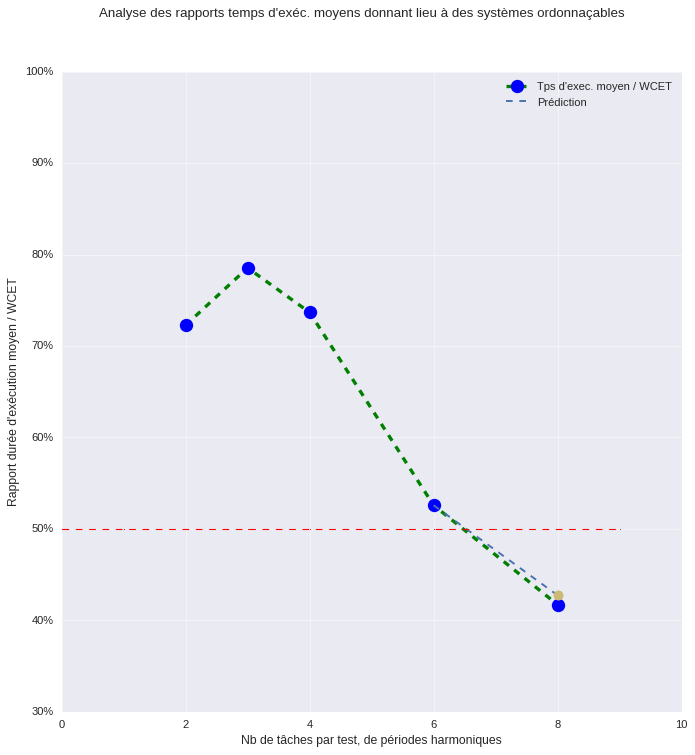
\includegraphics[scale=0.6]{img/wcet/wcetstudy}
		\end{figure}
	\end{center}
	
	Les conclusions par rapport à ces premiers tests sont de plusieurs ordres. 
	\begin{itemize}
		\item Tout d'abord, on observe que pour un petit nombre de tâches, les WCET ne sont pas très pessimistes par rapport aux temps d'exécutions moyens, 
		ce qui indique que l'algorithme donne de bonnes performances.
		\item En faisant varier le nombre de tâches, on observe cependant vite que la courbe tend vers le bas, et que les WCET deviennent 
		de plus en plus pessimistes.
		\item Pour 8 tâches, avec 8 périodes harmoniques, la prédiction faite s'est révélée très proche de la réalité, 
		ce qui nous a permis de construire un ensemble très rapidement.
	\end{itemize}

	Nous effectuons un dernier test avec une \textit{utilisation }de $100\%$ afin 
	de vérifier une hypothèse : en faisant des ensembles de périodes égales.
	
	\subsubsection{Périodes égales}
	
	\subsubsection{Évolution des temps dans l'ordonnanceur}
	
	Nous avons ajouté des \textit{logs} dans \textbf{HIPPEROS}, et ce faisant, nous procédons à une sorte de 
	profilage du code. Les temps que nous exposons ici sont une somme délivrée toutes les $60$ secondes environ 
	(cette fréquence est faible pour éviter de générer du surcoût supplémentaire avec des productions de sorties).
	
	
	\subsection{Utilisation 200 \%}
	
	Nous avons montré au chapitre Contexte que certains ensembles en théorie devraient être 
	ordonnançables par \textbf{UEDF }mais pas par\textbf{ Global-EDF}. Nous avons testé cet ensemble, sur les deux 
	ordonnanceurs. Pour ce faire, nous avons d'abord testé cet ensemble avec \textbf{UEDF }afin de paramétrer les WCET 
	de manière à ce que l'exécution ne génère pas de dépassements. Cet ensemble est en effet faisable, à condition 
	d'être pessimiste sur les WCET, c'est à dire avoir des temps moyens d'exécution des tâches éloignés de plus de la 
	moitié des WCET. \newline
	Nous avons voulu vérifier qu'en faisant varier la période (en la multipliant par $2$ puis par $3$) des tâches, 
	nous pouvions améliorer ce résultat, mais les tests ne nous ont pas montré cela, cette proportion semble 
	assez constante, comme le montre le tableau suivant. \newline
	
	\todo{inclure graph}
	
	Le plus étonnant est qu'avec ce paramétrage, l'ensemble devient ordonnçable par \textbf{Global-EDF}. 
	Pire encore, nous avons même le loisir d'augmenter la durée moyenne d'exécution des tâches et 
	l'ensemble reste ordonnaçable, comme le montre ce graphique. \newline
	
	Ce résultat montre le fossé qu'il peut y avoir ici entre la théorie, et la pratique, ce qui 
	s'explique facilement par le fait que certains paramètres sont considérés comme stables 
	voire indépendants, alors qu'en pratique, ils ne le sont pas forcément. \newline
	
	Il n'est pas absolument certain que des bugs viennent également minimiser les résultats, malgré notre 
	attention, il est possible que des erreurs subsistent. Cependant, en l'état, nous ne pouvons que constater le décalage 
	entre notre implémentation et le résultat théorique attendu, pour cet ensemble, et sans doute pour d'autres, 
	de périodes non harmoniques.\newline
	
	REMARQUE : la différence s'explique par le fait que lors d'un relâchement de tâches, 
	le set est réordonné, et que ce faisant, on provoque une préemption là où ce n'est pas 
	"nécessaire".
	
	Ceci peut expliquer l'augmentation importante du surcout.
	
	D'ailleurs, que nous disent les chiffres ??
	
	
	\todo{citation sur théorie/pratique/optimalité}
	
	\todo{inclure graph}
	
	Les temps d'appel à l'algorithme devant être à peu près constants, nous pouvons émettre l'hypothèse que le nombre 
	de migrations -- élevé pour cet ensemble -- est en partie responsable de ce résultat. Nous préciserons dans le chapitre suivant 
	comment remédier à ce problème dans le futur.\newline
	
	Ces expériences ont aiguillé la suite des études vers des ensembles de tâches de périodes harmoniques uniquement.

\section{Résultats quant à la faisabilité dans l'industrie}

	

\section{Résultats des tests unitaires et sur board}

	

\section{Comparaison avec G-EDF}

	